% Created by tikzDevice version 0.12.3.1 on 2022-08-11 16:48:57
% !TEX encoding = UTF-8 Unicode
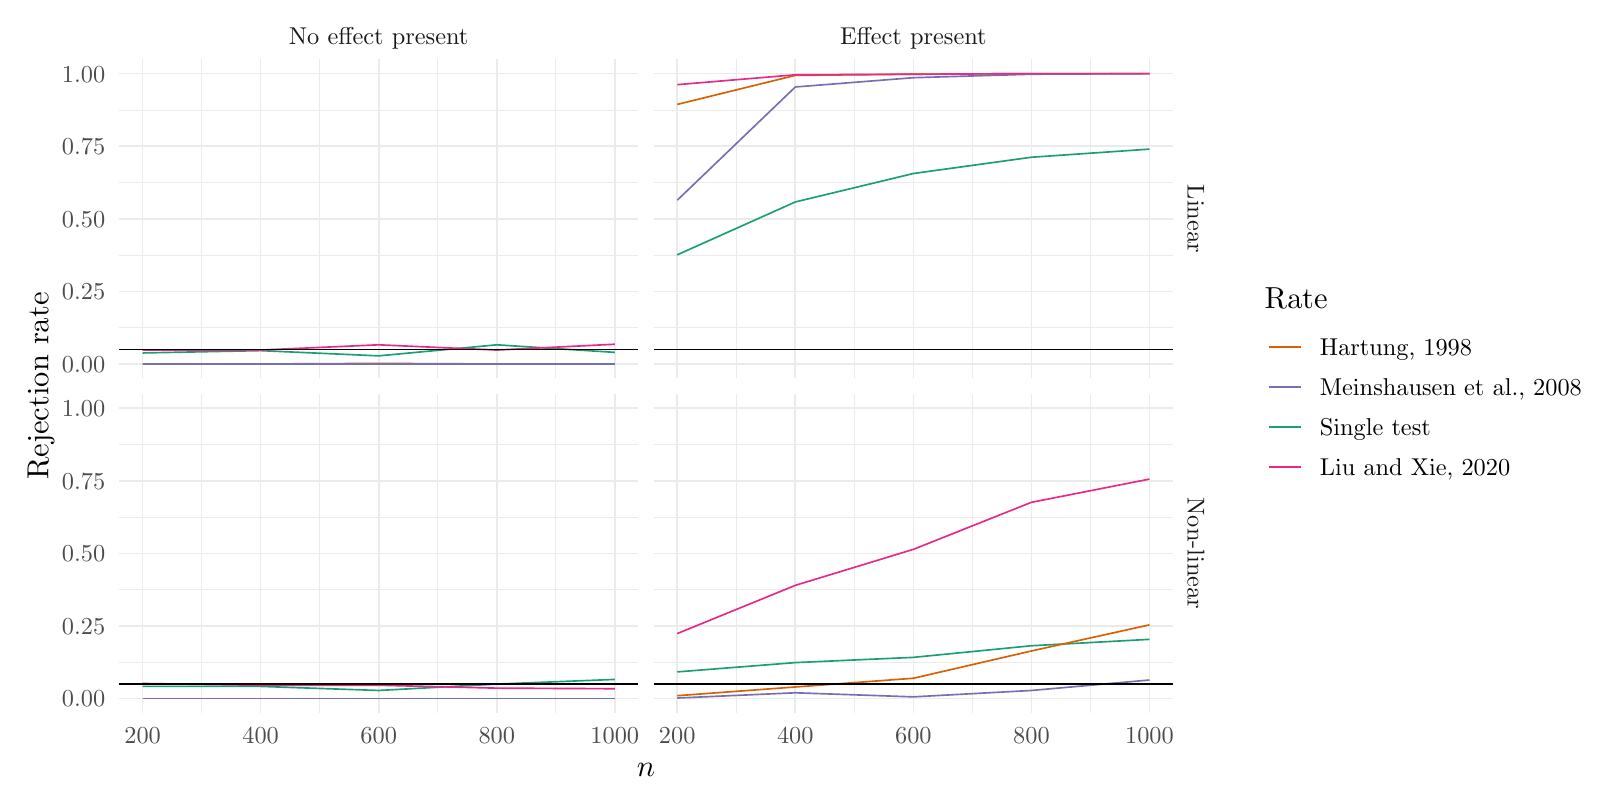
\begin{tikzpicture}[x=1pt,y=1pt]
\definecolor{fillColor}{RGB}{255,255,255}
\begin{scope}
\definecolor{drawColor}{gray}{0.92}

\path[draw=drawColor,line width= 0.3pt,line join=round] ( 38.56,169.96) --
	(226.26,169.96);

\path[draw=drawColor,line width= 0.3pt,line join=round] ( 38.56,196.19) --
	(226.26,196.19);

\path[draw=drawColor,line width= 0.3pt,line join=round] ( 38.56,222.42) --
	(226.26,222.42);

\path[draw=drawColor,line width= 0.3pt,line join=round] ( 38.56,248.65) --
	(226.26,248.65);

\path[draw=drawColor,line width= 0.3pt,line join=round] ( 68.42,151.60) --
	( 68.42,267.01);

\path[draw=drawColor,line width= 0.3pt,line join=round] (111.08,151.60) --
	(111.08,267.01);

\path[draw=drawColor,line width= 0.3pt,line join=round] (153.74,151.60) --
	(153.74,267.01);

\path[draw=drawColor,line width= 0.3pt,line join=round] (196.40,151.60) --
	(196.40,267.01);

\path[draw=drawColor,line width= 0.6pt,line join=round] ( 38.56,156.84) --
	(226.26,156.84);

\path[draw=drawColor,line width= 0.6pt,line join=round] ( 38.56,183.07) --
	(226.26,183.07);

\path[draw=drawColor,line width= 0.6pt,line join=round] ( 38.56,209.30) --
	(226.26,209.30);

\path[draw=drawColor,line width= 0.6pt,line join=round] ( 38.56,235.53) --
	(226.26,235.53);

\path[draw=drawColor,line width= 0.6pt,line join=round] ( 38.56,261.76) --
	(226.26,261.76);

\path[draw=drawColor,line width= 0.6pt,line join=round] ( 47.09,151.60) --
	( 47.09,267.01);

\path[draw=drawColor,line width= 0.6pt,line join=round] ( 89.75,151.60) --
	( 89.75,267.01);

\path[draw=drawColor,line width= 0.6pt,line join=round] (132.41,151.60) --
	(132.41,267.01);

\path[draw=drawColor,line width= 0.6pt,line join=round] (175.07,151.60) --
	(175.07,267.01);

\path[draw=drawColor,line width= 0.6pt,line join=round] (217.73,151.60) --
	(217.73,267.01);
\definecolor{drawColor}{RGB}{27,158,119}

\path[draw=drawColor,line width= 0.6pt,line join=round] ( 47.09,160.83) --
	( 89.75,161.67) --
	(132.41,159.78) --
	(175.07,163.77) --
	(217.73,161.04);
\definecolor{drawColor}{RGB}{217,95,2}

\path[draw=drawColor,line width= 0.6pt,line join=round] ( 47.09,156.84) --
	( 89.75,156.84) --
	(132.41,157.05) --
	(175.07,156.84) --
	(217.73,156.84);
\definecolor{drawColor}{RGB}{117,112,179}

\path[draw=drawColor,line width= 0.6pt,line join=round] ( 47.09,156.84) --
	( 89.75,156.84) --
	(132.41,156.84) --
	(175.07,156.84) --
	(217.73,156.84);
\definecolor{drawColor}{RGB}{231,41,138}

\path[draw=drawColor,line width= 0.6pt,line join=round] ( 47.09,161.88) --
	( 89.75,161.88) --
	(132.41,163.77) --
	(175.07,161.88) --
	(217.73,163.98);
\definecolor{drawColor}{RGB}{0,0,0}

\path[draw=drawColor,line width= 0.6pt,line join=round] ( 38.56,162.09) -- (226.26,162.09);
\end{scope}
\begin{scope}
\definecolor{drawColor}{gray}{0.92}

\path[draw=drawColor,line width= 0.3pt,line join=round] ( 38.56, 49.05) --
	(226.26, 49.05);

\path[draw=drawColor,line width= 0.3pt,line join=round] ( 38.56, 75.28) --
	(226.26, 75.28);

\path[draw=drawColor,line width= 0.3pt,line join=round] ( 38.56,101.51) --
	(226.26,101.51);

\path[draw=drawColor,line width= 0.3pt,line join=round] ( 38.56,127.74) --
	(226.26,127.74);

\path[draw=drawColor,line width= 0.3pt,line join=round] ( 68.42, 30.69) --
	( 68.42,146.10);

\path[draw=drawColor,line width= 0.3pt,line join=round] (111.08, 30.69) --
	(111.08,146.10);

\path[draw=drawColor,line width= 0.3pt,line join=round] (153.74, 30.69) --
	(153.74,146.10);

\path[draw=drawColor,line width= 0.3pt,line join=round] (196.40, 30.69) --
	(196.40,146.10);

\path[draw=drawColor,line width= 0.6pt,line join=round] ( 38.56, 35.93) --
	(226.26, 35.93);

\path[draw=drawColor,line width= 0.6pt,line join=round] ( 38.56, 62.16) --
	(226.26, 62.16);

\path[draw=drawColor,line width= 0.6pt,line join=round] ( 38.56, 88.39) --
	(226.26, 88.39);

\path[draw=drawColor,line width= 0.6pt,line join=round] ( 38.56,114.62) --
	(226.26,114.62);

\path[draw=drawColor,line width= 0.6pt,line join=round] ( 38.56,140.85) --
	(226.26,140.85);

\path[draw=drawColor,line width= 0.6pt,line join=round] ( 47.09, 30.69) --
	( 47.09,146.10);

\path[draw=drawColor,line width= 0.6pt,line join=round] ( 89.75, 30.69) --
	( 89.75,146.10);

\path[draw=drawColor,line width= 0.6pt,line join=round] (132.41, 30.69) --
	(132.41,146.10);

\path[draw=drawColor,line width= 0.6pt,line join=round] (175.07, 30.69) --
	(175.07,146.10);

\path[draw=drawColor,line width= 0.6pt,line join=round] (217.73, 30.69) --
	(217.73,146.10);
\definecolor{drawColor}{RGB}{27,158,119}

\path[draw=drawColor,line width= 0.6pt,line join=round] ( 47.09, 40.34) --
	( 89.75, 40.34) --
	(132.41, 38.87) --
	(175.07, 41.18) --
	(217.73, 42.86);
\definecolor{drawColor}{RGB}{217,95,2}

\path[draw=drawColor,line width= 0.6pt,line join=round] ( 47.09, 35.93) --
	( 89.75, 35.93) --
	(132.41, 35.93) --
	(175.07, 35.93) --
	(217.73, 35.93);
\definecolor{drawColor}{RGB}{117,112,179}

\path[draw=drawColor,line width= 0.6pt,line join=round] ( 47.09, 35.93) --
	( 89.75, 35.93) --
	(132.41, 35.93) --
	(175.07, 35.93) --
	(217.73, 35.93);
\definecolor{drawColor}{RGB}{231,41,138}

\path[draw=drawColor,line width= 0.6pt,line join=round] ( 47.09, 41.39) --
	( 89.75, 40.76) --
	(132.41, 40.76) --
	(175.07, 39.71) --
	(217.73, 39.50);
\definecolor{drawColor}{RGB}{0,0,0}

\path[draw=drawColor,line width= 0.6pt,line join=round] ( 38.56, 41.18) -- (226.26, 41.18);
\end{scope}
\begin{scope}
\definecolor{drawColor}{gray}{0.92}

\path[draw=drawColor,line width= 0.3pt,line join=round] (231.76,169.96) --
	(419.46,169.96);

\path[draw=drawColor,line width= 0.3pt,line join=round] (231.76,196.19) --
	(419.46,196.19);

\path[draw=drawColor,line width= 0.3pt,line join=round] (231.76,222.42) --
	(419.46,222.42);

\path[draw=drawColor,line width= 0.3pt,line join=round] (231.76,248.65) --
	(419.46,248.65);

\path[draw=drawColor,line width= 0.3pt,line join=round] (261.62,151.60) --
	(261.62,267.01);

\path[draw=drawColor,line width= 0.3pt,line join=round] (304.28,151.60) --
	(304.28,267.01);

\path[draw=drawColor,line width= 0.3pt,line join=round] (346.94,151.60) --
	(346.94,267.01);

\path[draw=drawColor,line width= 0.3pt,line join=round] (389.60,151.60) --
	(389.60,267.01);

\path[draw=drawColor,line width= 0.6pt,line join=round] (231.76,156.84) --
	(419.46,156.84);

\path[draw=drawColor,line width= 0.6pt,line join=round] (231.76,183.07) --
	(419.46,183.07);

\path[draw=drawColor,line width= 0.6pt,line join=round] (231.76,209.30) --
	(419.46,209.30);

\path[draw=drawColor,line width= 0.6pt,line join=round] (231.76,235.53) --
	(419.46,235.53);

\path[draw=drawColor,line width= 0.6pt,line join=round] (231.76,261.76) --
	(419.46,261.76);

\path[draw=drawColor,line width= 0.6pt,line join=round] (240.29,151.60) --
	(240.29,267.01);

\path[draw=drawColor,line width= 0.6pt,line join=round] (282.95,151.60) --
	(282.95,267.01);

\path[draw=drawColor,line width= 0.6pt,line join=round] (325.61,151.60) --
	(325.61,267.01);

\path[draw=drawColor,line width= 0.6pt,line join=round] (368.27,151.60) --
	(368.27,267.01);

\path[draw=drawColor,line width= 0.6pt,line join=round] (410.93,151.60) --
	(410.93,267.01);
\definecolor{drawColor}{RGB}{27,158,119}

\path[draw=drawColor,line width= 0.6pt,line join=round] (240.29,196.29) --
	(282.95,215.39) --
	(325.61,225.67) --
	(368.27,231.55) --
	(410.93,234.48);
\definecolor{drawColor}{RGB}{217,95,2}

\path[draw=drawColor,line width= 0.6pt,line join=round] (240.29,250.64) --
	(282.95,261.13) --
	(325.61,261.55) --
	(368.27,261.76) --
	(410.93,261.76);
\definecolor{drawColor}{RGB}{117,112,179}

\path[draw=drawColor,line width= 0.6pt,line join=round] (240.29,216.02) --
	(282.95,256.94) --
	(325.61,260.29) --
	(368.27,261.55) --
	(410.93,261.76);
\definecolor{drawColor}{RGB}{231,41,138}

\path[draw=drawColor,line width= 0.6pt,line join=round] (240.29,257.78) --
	(282.95,261.34) --
	(325.61,261.55) --
	(368.27,261.76) --
	(410.93,261.76);
\definecolor{drawColor}{RGB}{0,0,0}

\path[draw=drawColor,line width= 0.6pt,line join=round] (231.76,162.09) -- (419.46,162.09);
\end{scope}
\begin{scope}
\definecolor{drawColor}{gray}{0.92}

\path[draw=drawColor,line width= 0.3pt,line join=round] (231.76, 49.05) --
	(419.46, 49.05);

\path[draw=drawColor,line width= 0.3pt,line join=round] (231.76, 75.28) --
	(419.46, 75.28);

\path[draw=drawColor,line width= 0.3pt,line join=round] (231.76,101.51) --
	(419.46,101.51);

\path[draw=drawColor,line width= 0.3pt,line join=round] (231.76,127.74) --
	(419.46,127.74);

\path[draw=drawColor,line width= 0.3pt,line join=round] (261.62, 30.69) --
	(261.62,146.10);

\path[draw=drawColor,line width= 0.3pt,line join=round] (304.28, 30.69) --
	(304.28,146.10);

\path[draw=drawColor,line width= 0.3pt,line join=round] (346.94, 30.69) --
	(346.94,146.10);

\path[draw=drawColor,line width= 0.3pt,line join=round] (389.60, 30.69) --
	(389.60,146.10);

\path[draw=drawColor,line width= 0.6pt,line join=round] (231.76, 35.93) --
	(419.46, 35.93);

\path[draw=drawColor,line width= 0.6pt,line join=round] (231.76, 62.16) --
	(419.46, 62.16);

\path[draw=drawColor,line width= 0.6pt,line join=round] (231.76, 88.39) --
	(419.46, 88.39);

\path[draw=drawColor,line width= 0.6pt,line join=round] (231.76,114.62) --
	(419.46,114.62);

\path[draw=drawColor,line width= 0.6pt,line join=round] (231.76,140.85) --
	(419.46,140.85);

\path[draw=drawColor,line width= 0.6pt,line join=round] (240.29, 30.69) --
	(240.29,146.10);

\path[draw=drawColor,line width= 0.6pt,line join=round] (282.95, 30.69) --
	(282.95,146.10);

\path[draw=drawColor,line width= 0.6pt,line join=round] (325.61, 30.69) --
	(325.61,146.10);

\path[draw=drawColor,line width= 0.6pt,line join=round] (368.27, 30.69) --
	(368.27,146.10);

\path[draw=drawColor,line width= 0.6pt,line join=round] (410.93, 30.69) --
	(410.93,146.10);
\definecolor{drawColor}{RGB}{27,158,119}

\path[draw=drawColor,line width= 0.6pt,line join=round] (240.29, 45.58) --
	(282.95, 48.94) --
	(325.61, 50.83) --
	(368.27, 55.03) --
	(410.93, 57.34);
\definecolor{drawColor}{RGB}{217,95,2}

\path[draw=drawColor,line width= 0.6pt,line join=round] (240.29, 36.98) --
	(282.95, 40.13) --
	(325.61, 43.28) --
	(368.27, 53.14) --
	(410.93, 62.58);
\definecolor{drawColor}{RGB}{117,112,179}

\path[draw=drawColor,line width= 0.6pt,line join=round] (240.29, 36.14) --
	(282.95, 38.03) --
	(325.61, 36.56) --
	(368.27, 38.87) --
	(410.93, 42.65);
\definecolor{drawColor}{RGB}{231,41,138}

\path[draw=drawColor,line width= 0.6pt,line join=round] (240.29, 59.43) --
	(282.95, 76.85) --
	(325.61, 89.86) --
	(368.27,106.86) --
	(410.93,115.25);
\definecolor{drawColor}{RGB}{0,0,0}

\path[draw=drawColor,line width= 0.6pt,line join=round] (231.76, 41.18) -- (419.46, 41.18);
\end{scope}
\begin{scope}
\definecolor{drawColor}{gray}{0.10}

\node[text=drawColor,anchor=base,inner sep=0pt, outer sep=0pt, scale=  0.88] at (132.41,272.26) {No effect present};
\end{scope}
\begin{scope}
\definecolor{drawColor}{gray}{0.10}

\node[text=drawColor,anchor=base,inner sep=0pt, outer sep=0pt, scale=  0.88] at (325.61,272.26) {Effect present};
\end{scope}
\begin{scope}
\definecolor{drawColor}{gray}{0.10}

\node[text=drawColor,rotate=-90.00,anchor=base,inner sep=0pt, outer sep=0pt, scale=  0.88] at (424.71,209.30) {Linear};
\end{scope}
\begin{scope}
\definecolor{drawColor}{gray}{0.10}

\node[text=drawColor,rotate=-90.00,anchor=base,inner sep=0pt, outer sep=0pt, scale=  0.88] at (424.71, 88.39) {Non-linear};
\end{scope}
\begin{scope}
\definecolor{drawColor}{gray}{0.30}

\node[text=drawColor,anchor=base,inner sep=0pt, outer sep=0pt, scale=  0.88] at ( 47.09, 19.68) {200};

\node[text=drawColor,anchor=base,inner sep=0pt, outer sep=0pt, scale=  0.88] at ( 89.75, 19.68) {400};

\node[text=drawColor,anchor=base,inner sep=0pt, outer sep=0pt, scale=  0.88] at (132.41, 19.68) {600};

\node[text=drawColor,anchor=base,inner sep=0pt, outer sep=0pt, scale=  0.88] at (175.07, 19.68) {800};

\node[text=drawColor,anchor=base,inner sep=0pt, outer sep=0pt, scale=  0.88] at (217.73, 19.68) {1000};
\end{scope}
\begin{scope}
\definecolor{drawColor}{gray}{0.30}

\node[text=drawColor,anchor=base,inner sep=0pt, outer sep=0pt, scale=  0.88] at (240.29, 19.68) {200};

\node[text=drawColor,anchor=base,inner sep=0pt, outer sep=0pt, scale=  0.88] at (282.95, 19.68) {400};

\node[text=drawColor,anchor=base,inner sep=0pt, outer sep=0pt, scale=  0.88] at (325.61, 19.68) {600};

\node[text=drawColor,anchor=base,inner sep=0pt, outer sep=0pt, scale=  0.88] at (368.27, 19.68) {800};

\node[text=drawColor,anchor=base,inner sep=0pt, outer sep=0pt, scale=  0.88] at (410.93, 19.68) {1000};
\end{scope}
\begin{scope}
\definecolor{drawColor}{gray}{0.30}

\node[text=drawColor,anchor=base east,inner sep=0pt, outer sep=0pt, scale=  0.88] at ( 33.61,153.81) {0.00};

\node[text=drawColor,anchor=base east,inner sep=0pt, outer sep=0pt, scale=  0.88] at ( 33.61,180.04) {0.25};

\node[text=drawColor,anchor=base east,inner sep=0pt, outer sep=0pt, scale=  0.88] at ( 33.61,206.27) {0.50};

\node[text=drawColor,anchor=base east,inner sep=0pt, outer sep=0pt, scale=  0.88] at ( 33.61,232.50) {0.75};

\node[text=drawColor,anchor=base east,inner sep=0pt, outer sep=0pt, scale=  0.88] at ( 33.61,258.73) {1.00};
\end{scope}
\begin{scope}
\definecolor{drawColor}{gray}{0.30}

\node[text=drawColor,anchor=base east,inner sep=0pt, outer sep=0pt, scale=  0.88] at ( 33.61, 32.90) {0.00};

\node[text=drawColor,anchor=base east,inner sep=0pt, outer sep=0pt, scale=  0.88] at ( 33.61, 59.13) {0.25};

\node[text=drawColor,anchor=base east,inner sep=0pt, outer sep=0pt, scale=  0.88] at ( 33.61, 85.36) {0.50};

\node[text=drawColor,anchor=base east,inner sep=0pt, outer sep=0pt, scale=  0.88] at ( 33.61,111.59) {0.75};

\node[text=drawColor,anchor=base east,inner sep=0pt, outer sep=0pt, scale=  0.88] at ( 33.61,137.82) {1.00};
\end{scope}
\begin{scope}
\definecolor{drawColor}{RGB}{0,0,0}

\node[text=drawColor,anchor=base,inner sep=0pt, outer sep=0pt, scale=  1.10] at (229.01,  7.64) {$n$};
\end{scope}
\begin{scope}
\definecolor{drawColor}{RGB}{0,0,0}

\node[text=drawColor,rotate= 90.00,anchor=base,inner sep=0pt, outer sep=0pt, scale=  1.10] at ( 13.08,148.85) {Rejection rate};
\end{scope}
\begin{scope}
\definecolor{drawColor}{RGB}{0,0,0}

\node[text=drawColor,anchor=base west,inner sep=0pt, outer sep=0pt, scale=  1.10] at (452.53,176.72) {Rate};
\end{scope}
\begin{scope}
\definecolor{drawColor}{RGB}{217,95,2}

\path[draw=drawColor,line width= 0.6pt,line join=round] (453.98,162.92) -- (465.54,162.92);
\end{scope}
\begin{scope}
\definecolor{drawColor}{RGB}{117,112,179}

\path[draw=drawColor,line width= 0.6pt,line join=round] (453.98,148.47) -- (465.54,148.47);
\end{scope}
\begin{scope}
\definecolor{drawColor}{RGB}{27,158,119}

\path[draw=drawColor,line width= 0.6pt,line join=round] (453.98,134.01) -- (465.54,134.01);
\end{scope}
\begin{scope}
\definecolor{drawColor}{RGB}{231,41,138}

\path[draw=drawColor,line width= 0.6pt,line join=round] (453.98,119.56) -- (465.54,119.56);
\end{scope}
\begin{scope}
\definecolor{drawColor}{RGB}{0,0,0}

\node[text=drawColor,anchor=base west,inner sep=0pt, outer sep=0pt, scale=  0.88] at (472.48,159.89) {Hartung, 1998};
\end{scope}
\begin{scope}
\definecolor{drawColor}{RGB}{0,0,0}

\node[text=drawColor,anchor=base west,inner sep=0pt, outer sep=0pt, scale=  0.88] at (472.48,145.44) {Meinshausen et al., 2008};
\end{scope}
\begin{scope}
\definecolor{drawColor}{RGB}{0,0,0}

\node[text=drawColor,anchor=base west,inner sep=0pt, outer sep=0pt, scale=  0.88] at (472.48,130.98) {Single test};
\end{scope}
\begin{scope}
\definecolor{drawColor}{RGB}{0,0,0}

\node[text=drawColor,anchor=base west,inner sep=0pt, outer sep=0pt, scale=  0.88] at (472.48,116.53) {Liu and Xie, 2020};
\end{scope}
\end{tikzpicture}
